\chapter{Projeto Conceitual do Produto}

\section{Características gerais}

\textcolor{red}{Descrever produto de forma geral. Apresentar itens teóricos sobre o projeto a serem aprofundados ou detalhados oportunamente.}

\textcolor{red}{Apresentar e explicar a Estrutura Analítica do Projeto (EAP), tomando cuidado com a legibilidade da imagem. Se necessário, coloque a EAP dentro do comando ``\textsf{\textbackslash begin\{landscape\} \textbackslash end\{landscape\}}'' para que ela seja apresentada em uma página deitada.}

\section{Estrutura}

\textcolor{red}{Apresentar desenho em CAD, indicar dimensões por lado/aresta/cota, indicar materiais utilizados e explicar o desenho e as decisões de projeto.}

\section{Descrição de \textit{hardware}}

A presente seção detalha a arquitetura de hardware desenvolvida para o micromouse XAROPi. A descrição a seguir permite a compreensão e a plena replicação do produto proposto neste documento. Para isso, os subsistemas principais e as escolhas de projeto são explicados de forma textual, acompanhados da lista completa de componentes, do diagrama de blocos e, por fim, do esquema elétrico das conexões. \\

Para a concretização do projeto físico, foram selecionados componentes que equilibram custo, disponibilidade e desempenho para os requisitos de navegação autônoma. A Tabela \ref{tab:lista_materiais} apresenta a lista de materiais principal utilizada no chassi do robô.

\begin{table}[H]
    \centering
    \caption{Lista de materiais do Micromouse.}
    \label{tab:lista_materiais}
    \resizebox{\textwidth}{!}{%
    \begin{tabular}{|l|l|c|p{5cm}|}
        \hline
        \textbf{Componente} & \textbf{Modelo} & \textbf{Qtd.} & \textbf{Descrição} \\
        \hline
        Microcontrolador & ESP32-S3-WROOM-1-N16R8 & 1 & Responsável pelo processamento do algoritmo de navegação e telemetria. \\
        \hline
        Sensor de Distância (ToF) & VL53L0X & 3 & Mapeamento frontal e lateral das paredes do labirinto. \\
        \hline
        Sensor Inercial & MPU-6000 & 1 & Acelerômetro e giroscópio de 6 eixos para controle de orientação. \\
        \hline
        Micro Motor DC com Encoder & 6V-750RPM & 2 & Motores com caixas de redução e encoders de quadratura integrados. \\
        \hline
        Driver de Potência (Ponte H) & L298N & 1 & Módulo Ponte H baseado no CI L298N. \\
        \hline
        BMS & BMS-20A-3S-S & 1 & Módulo BMS (Battery Management System). \\
        \hline
        Regulador de Tensão (Step-down) & LM2596 & 1 & Fornece a tensão lógica adequada aos periféricos e ao microcontrolador. \\
        \hline
    \end{tabular}}
\end{table}
A Figura \ref{fig:diagrama_componentes}  apresenta o diagrama de blocos do sistema, ilustrando o fluxo de energia e a troca de dados entre os componentes. A arquitetura do robô é dividida logicamente em dois domínios principais: o subsistema de potência e o subsistema de controle e comunicação.

No subsistema de alimentação, a energia fornecida pela bateria passa inicialmente pelo módulo BMS, responsável por proteger e garantir a integridade das células de lítio. Em seguida, o circuito é dividido em duas vias principais: uma linha de alta potência conectada diretamente à Ponte H, capaz de suprir a corrente exigida pelos motores, e uma linha secundária regulada pelo módulo LM2596. Este regulador reduz e estabiliza a tensão para alimentar de forma segura o microcontrolador ESP32-S3 e os sensores periféricos.

O gerenciamento de todo o sistema é centralizado no ESP32-S3. Ele opera como o dispositivo mestre, realizando a leitura contínua dos dados do módulo inercial e dos sensores ToF por meio de um barramento de comunicação digital. A movimentação do robô ocorre sob um controle em malha fechada: o microcontrolador envia os comandos de atuação (PWM e direção) para a Ponte H e, simultaneamente, recebe o feedback odométrico por meio das interrupções geradas pelos encoders dos motores. Esse ciclo permite que o sistema calcule o deslocamento e ajuste a trajetória em tempo real.
\begin{figure}[H]
    \centering
    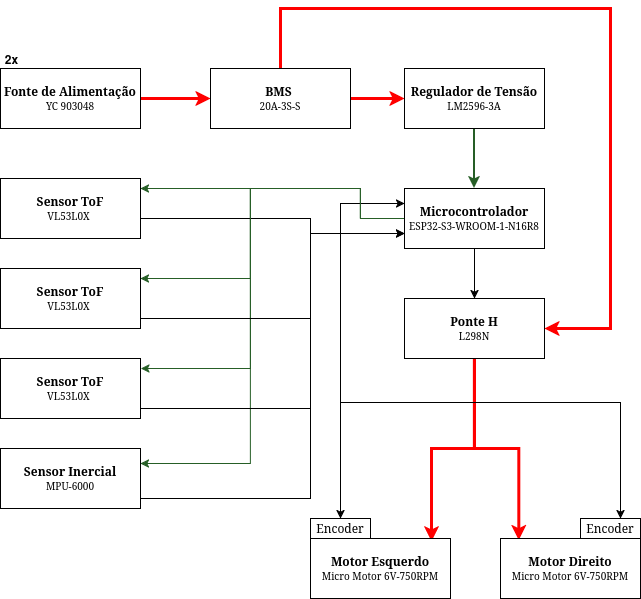
\includegraphics[width=0.8\textwidth]{figuras/diagrama_componentesFinal.png}
    \captionsetup{font=footnotesize}
    \caption{Diagrama de componentes do Micromouse. As linhas contínuas pretas representam conexões físicas via protocolo I2C. As linhas verdes representam alimentação em baixa tensão (3,3V). As linhas vermelhas representam alimentação em alta tensão (6V). As linhas tracejadas representam comunicação sem fio.}
    \label{fig:diagrama_componentes}
\end{figure}


\textcolor{red}{A Fig. \ref{fig:diagrama_blocos_e_esquematico} apresenta o diagrama de blocos e o esquemático de um circuito conversor de corrente alternada para corrente direta, a título de exemplo. Repare que o diagrama de blocos indica os subsistemas do circuito completo apresentado no esquemático.
% Comecem com o diagrama de blocos, que é mais genérico, e depois indiquem os detalhes com a lista de materiais e os esquemáticos.
}

\begin{figure}[H]
    \centering
    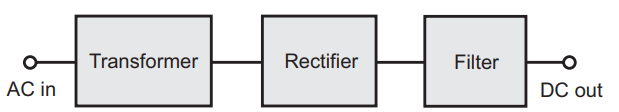
\includegraphics[width=0.5\linewidth]{figuras/Exemplo-diagrama-de-blocos.png}
    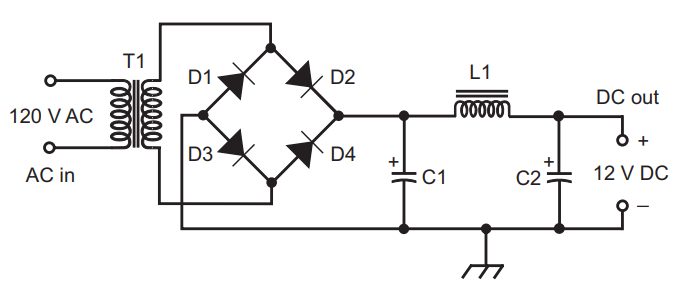
\includegraphics[width=0.5\linewidth]{figuras/Esquematico.png}
    \caption{\textcolor{red}{Diagrama de blocos e esquemático de um circuito conversor de corrente alternada para corrente direta. Extraído de \cite{block_n_schematic}.}}
    \label{fig:diagrama_blocos_e_esquematico}
\end{figure}

\section{Análise de consumo energético}

\textcolor{red}{Com relação ao consumo energético do produto desenvolvido, será necessário apresentar cálculos de consumo dos diversos componentes utilizados e explicar as decisões de projeto para atender a estas demandas.}


\begin{itemize}
    \item \textcolor{red}{ \textbf{Identificação dos Subsistemas Elétricos:} liste todos os componentes que consumirão energia, como sensores, microcontroladores, atuadores e módulos de armazenamento de dados. Para cada componente, registre a tensão de operação (V), corrente média (mA) e tempo estimado de uso (s).}
    \item \textcolor{red}{ \textbf{Cálculo da Energia Consumida por Componente:} utilize a fórmula: $E = V I t$, onde $E$ é a energia em joules, $V$ é a tensão em volts, $I$ a corrente em ampères e $t$ o tempo em segundos. Realize esse cálculo para cada componente do sistema.}
    \item \textcolor{red}{ \textbf{Estimativa do Consumo Total de Energia:} some as energias de todos os componentes para obter o consumo energético total estimado do sistema por lançamento.}
    \item \textcolor{red}{ \textbf{Escolha da Fonte de Alimentação:} com base no consumo total, converta para watt-hora: 1 Wh = 3600 J. Adicione e justifique uma margem de segurança (pesquisar o que é usual para este tipo de sistema) e selecione uma bateria ou fonte que supra a demanda.}
    \item \textcolor{red}{ \textbf{Planejamento do Circuito de Alimentação:} analise a necessidade de inclusão de reguladores de tensão, proteções contra sobrecorrente, e isolamento para atuadores. Como as oscilações de tensão serão controladas?}
    \item \textcolor{red}{ \textbf{Monitoramento via \textit{software}:} implemente, no \textit{software} embarcado, rotinas para medir a tensão da bateria e registrar dados de tempo de operação. Colete os dados para análise.}
    \item \textcolor{red}{ \textbf{Validação com Testes Reais:} realize testes de campo para comparar o consumo estimado com o real. Ajuste a capacidade da fonte se necessário e refine o software de coleta de dados. Justifique a diferença de resultados (real x teórica), de acordo com a literatura.}
\end{itemize}

\section{Descrição de \textit{software}}

\subsection{Diagrama de Atividades}

O Diagrama de Atividades (Figura \ref{fig:diagrama_atividades_sw}) descreve o comportamento funcional do sistema web do projeto XAROPi. A modelagem utiliza o particionamento por raias (\textit{swimlanes}) para estruturar o fluxo e evidenciar a fronteira entre os subsistemas da arquitetura.

Com base na notação UML, o fluxo destaca os seguintes elementos funcionais:
\begin{itemize}
    \item \textbf{Atores envolvidos:} O Estudante e o sistema físico do Micromouse.
    \item \textbf{Atividades de negócio:} Emissão de comandos de controle direcional, processamento da matriz lógica e renderização do trajeto.
    \item \textbf{Insumos (Entradas):} Ações diretas na interface pelo usuário e pacotes de telemetria transmitidos pelo ESP32 via protocolo WebSocket.
    \item \textbf{Resultados (Saídas):} Atualização dinâmica do mapa lógico na tela e a gravação final do histórico do percurso no Firebase.
    \item \textbf{Pontos de decisão:} O diagrama apresenta nós de verificação condicionais, especificamente na validação prévia de conexão estabelecida e na condição de parada automática.
\end{itemize}

O fluxo de controle se desenvolve a partir do nó de estado inicial, transitando pelas atividades assíncronas do \textit{loop} de atualização e permitindo sinais de interrupção manual pelo usuário, até o armazenamento dos dados e o atingimento do estado final.

\begin{figure}[H]
    \centering
    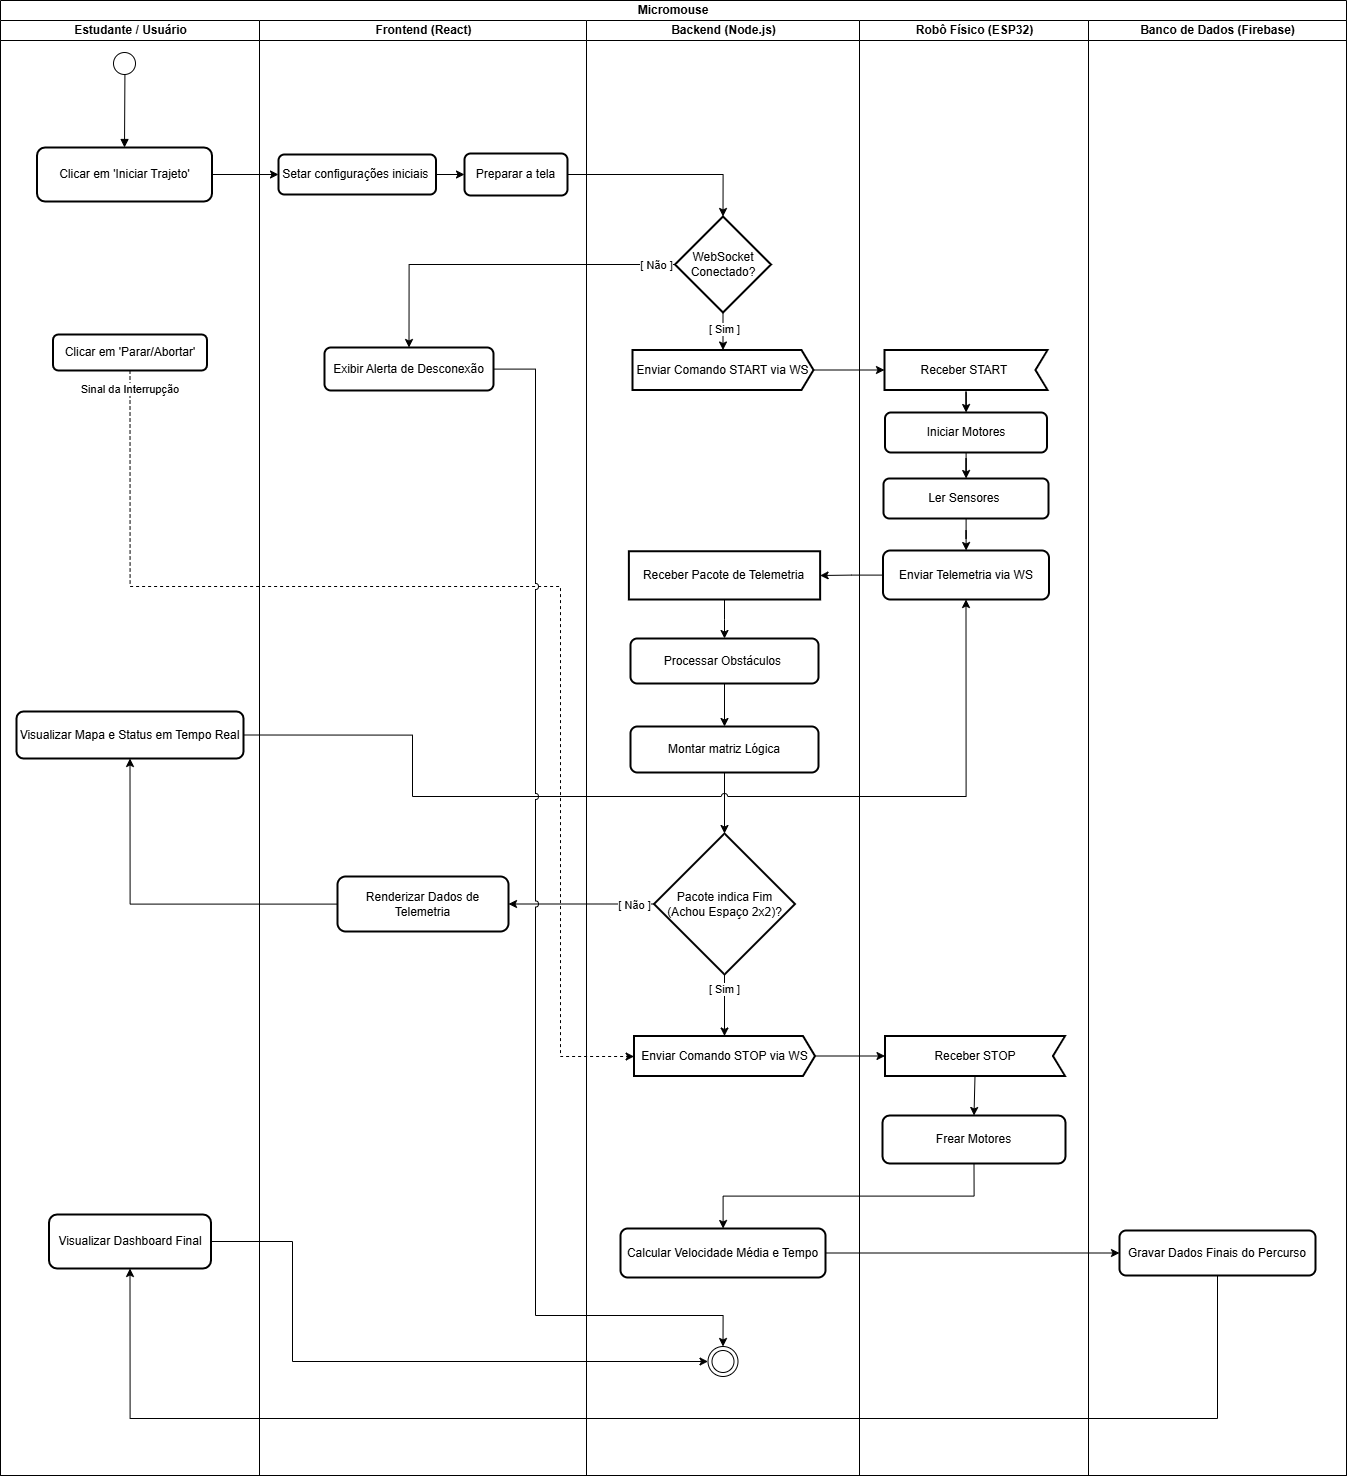
\includegraphics[height=15cm]{figuras/software/diagrama_atividades.png}
    \caption{Diagrama de Atividades de Software XAROPi.}
    \label{fig:diagrama_atividades_sw}
\end{figure}

\subsection{Backlog do Produto}

O backlog do produto é uma lista priorizada de requisitos e funcionalidades que guia o desenvolvimento do produto. Ele foi estruturado com base na EAP do projeto, (add numero da figura), e classificado utilizando a técnica MoSCoW para priorizar os requisitos e histórias de usuário. 
O backlog foi todo estruturado no github e pode ser acessado através deste \href{https://github.com/orgs/fcte-pi1/projects/8/views/1?visibleFields=%5B%22Title%22%2C274081113%2C274081114%2C%22Labels%22%2C%22Milestone%22%2C%22Assignees%22%2C%22Sub-issues+progress%22%2C%22Status%22%2C274081112%2C274081111%2C%22Linked+pull+requests%22%2C274111004%5D&hierarchy=true}{link}, onde é possivel observar com mais detalhes e compreender na sua totalidade o backlog do produto.

Na figura \ref{fig:backlog_produto} é possível observar um recorte do backlog do produto onde é possivel observar as releases, épicos, histórias de usuário e a prioriação. Além disto, cada HU está relacionada há uma parte do protótipo, ao acessar a issue específica de cada HU é possível observar na descrição. 

\begin{figure}[H]
    \centering
    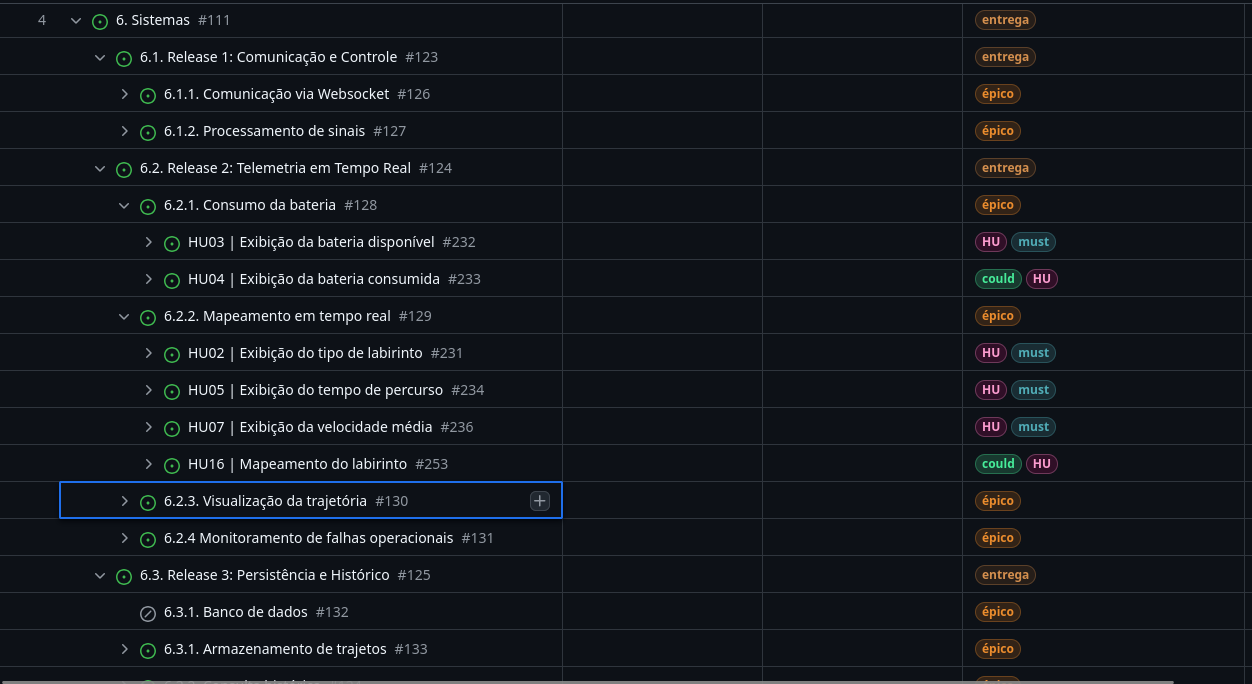
\includegraphics[width=\textwidth]{figuras/software/backlog.png}
    \captionsetup{font=footnotesize}
    \caption{Backlog do Produto (GitHub).}
    \label{fig:backlog_produto}
\end{figure}

\subsubsection{Protótipo Funcional}
O protótipo funcional foi desenvolvido com base nos requisitos funcionais que requerem apresentação e interação na interface, representados pelas Histórias do Usuário. Inicialmente, o protótipo possui duas páginas principais:
\begin{enumerate}
    \item \textbf{Página de Visão Geral:} Concentra as informações gerais de todos os testes, fornecendo métricas e gráficos importantes para uma visão holística dos testes executados. A implementação dessas funcionalidades serão essenciais para o monitoramento da evolução do projeto em uma perspectiva mais ampla Além disso, essa página também fornece uma tabela para consulta histórica dos dados de trajetos anteriores. Isso permitirá escolher quais recuperar informações de testes executados recuperar com uma visualização rápida. As HUs relacionadas a essa tela incluem: 
\href{https://github.com/fcte-pi1/2026.1_PI1_Grupo01_Bruno/issues/232}{HU03},  
\href{https://github.com/fcte-pi1/2026.1_PI1_Grupo01_Bruno/issues/233}{HU04}, 
\href{https://github.com/fcte-pi1/2026.1_PI1_Grupo01_Bruno/issues/248}{HU11}, 
\href{https://github.com/fcte-pi1/2026.1_PI1_Grupo01_Bruno/issues/249}{HU12}, 
\href{https://github.com/fcte-pi1/2026.1_PI1_Grupo01_Bruno/issues/250}{HU13}.
    \item \textbf{Página de Monitoramento em Tempo Real:} É a página a ser utilizada durante a execução de cada caso de teste. Ela exibe informações em tempo real enviadas pelo robô, como distância percorrida, obstáculos encontrados, gasto da bateria, bem como renderiza o mapa em tempo real conforme o \textit{Micromouse} o explora. Por fim, essa página também constrói e exibe gráficos como de velocidade e consumo energético. As HUs relacionadas incluem: 
\href{https://github.com/fcte-pi1/2026.1_PI1_Grupo01_Bruno/issues/230}{HU01}, 
\href{https://github.com/fcte-pi1/2026.1_PI1_Grupo01_Bruno/issues/231}{HU02}, 
\href{https://github.com/fcte-pi1/2026.1_PI1_Grupo01_Bruno/issues/234}{HU05},  
\href{https://github.com/fcte-pi1/2026.1_PI1_Grupo01_Bruno/issues/235}{HU06},  
\href{https://github.com/fcte-pi1/2026.1_PI1_Grupo01_Bruno/issues/236}{HU07}, 
\href{https://github.com/fcte-pi1/2026.1_PI1_Grupo01_Bruno/issues/237}{HU08}, 
\href{https://github.com/fcte-pi1/2026.1_PI1_Grupo01_Bruno/issues/246}{HU09},  
\href{https://github.com/fcte-pi1/2026.1_PI1_Grupo01_Bruno/issues/247}{HU10},  
\href{https://github.com/fcte-pi1/2026.1_PI1_Grupo01_Bruno/issues/251}{HU14},  
\href{https://github.com/fcte-pi1/2026.1_PI1_Grupo01_Bruno/issues/252}{HU15},  
\href{https://github.com/fcte-pi1/2026.1_PI1_Grupo01_Bruno/issues/253}{HU16};  
\end{enumerate}

\begin{figure}[H]
    \centering
    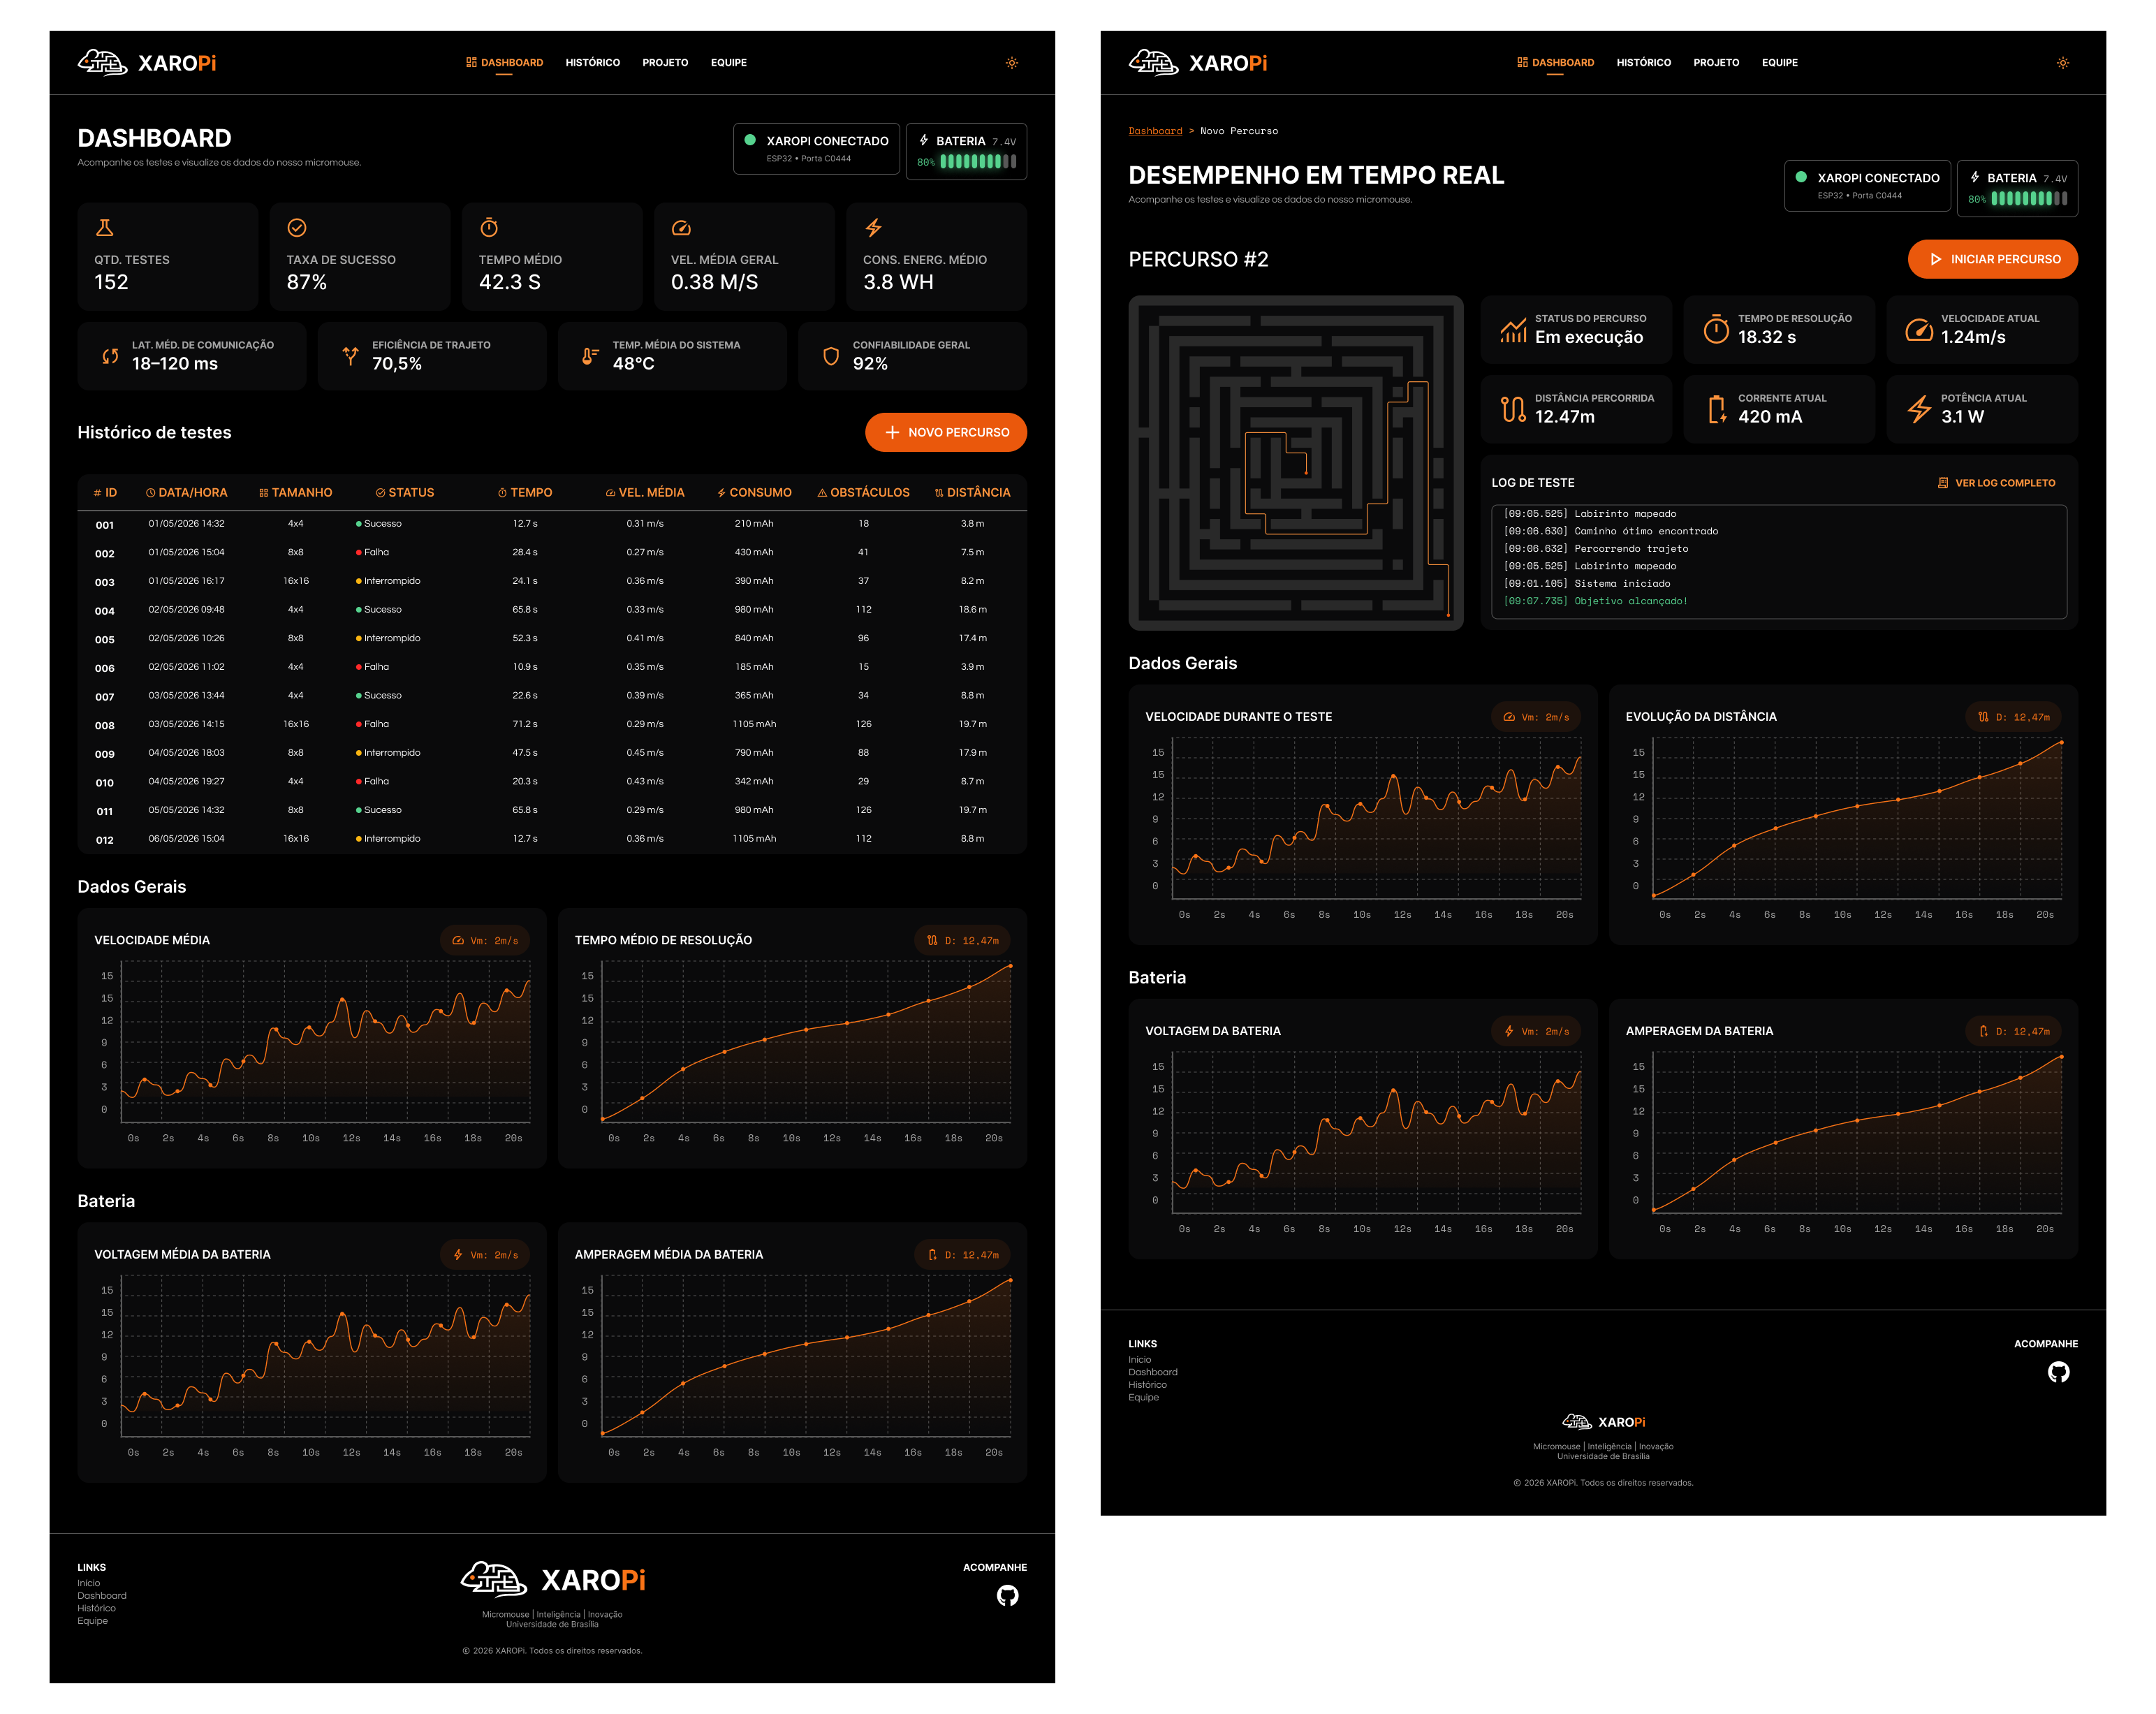
\includegraphics[width=\textwidth]{figuras/software/prototipo.png}
    \captionsetup{font=footnotesize}
    \caption{Protótipo Funcional do Sistema.}
    \label{fig:prototipo_funcional}
\end{figure}

\href{https://www.figma.com/proto/2ZyxT13T50XnVaUs51JKeb/XAROPi---Prot%C3%B3tipo-Funcional?page-id=0%3A1&node-id=46-1543&viewport=-1443%2C185%2C0.37&t=nvLNuJQbUXyazppG-1&scaling=min-zoom&content-scaling=fixed&starting-point-node-id=46%3A1543}{Link para acessar o protótipo navegável.}

\subsection{Descrição da Arquitetura do Software}

O propósito do software no projeto XAROPi é apresentar em um ambiente web e em tempo real os dados de telemetria do micromouse. Além disso, o sistema deve armazenar os dados das tentativas de resolução do labirinto e permitir consultas posteriores à finalização dos trajetos.

Para a viabilização dessas tarefas, optou-se por um modelo \textbf{monolítico em camadas}, com separação estrita entre a interface de usuário (\textit{frontend}), as lógicas de negócio (\textit{backend}) e a persistência de informações (banco de dados). A escolha pela arquitetura monolítica no lado do servidor justifica-se pela simplicidade de desenvolvimento e implantação, alinhando-se à curva de adaptação da equipe. A divisão lógica em camadas, por sua vez, garante a organização do código e facilita a manutenção.

O ecossistema do software é unificado pelo uso de \textit{JavaScript/TypeScript} e estruturado nas seguintes tecnologias e padrões:

\begin{itemize}
    \item \textbf{Interface (\textit{Frontend}):} Desenvolvida utilizando a biblioteca \textit{React}, operando com uma arquitetura orientada a componentes. A interface consome os dados do servidor e atualiza a visualização dinamicamente, separando a lógica de apresentação da lógica de processamento pesado.
    \item \textbf{Servidor (\textit{Backend}):} Construído em \textit{Node.js} com o \textit{framework} \textit{NestJS}. O \textit{backend} adota uma \textbf{Arquitetura Modular} (Controladores e Serviços), atuando como uma API que fornece dados via HTTP/REST e mantém comunicação de baixa latência com o robô via protocolo \textit{WebSocket}.
    \item \textbf{Banco de Dados:} Para o armazenamento das execuções, utiliza-se o \textit{Firebase}, um banco de dados \textit{NoSQL} orientado a documentos. Esta tecnologia permite gravar as matrizes do labirinto e tempos de percurso com alta flexibilidade e velocidade de consulta.
\end{itemize}

\subsubsection{Propósito do Software}
\subsubsection{Padrão adotado}
\subsubsection{Tecnologias escolhidas}

\subsection{Visão Lógica do Software}
\subsubsection{Diagrama de Classes}

A figura \ref{fig:diagrama_classes} apresenta o diagrama de classes do sistema, entre elas, classes para acesso ao banco de dados, para interpretação dos dados de telemetria para o frontend e para o recebimento e envio de dados com websocket. 

\begin{figure}[H]
    \centering
    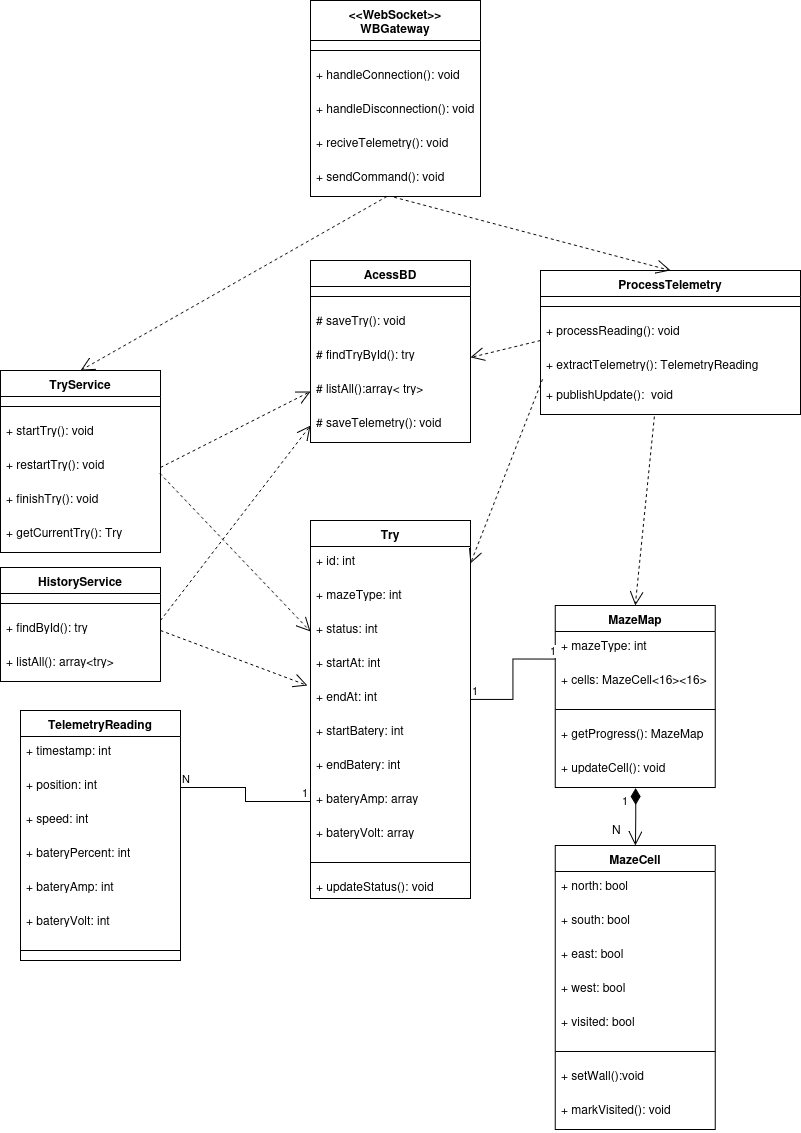
\includegraphics[height=15cm]{figuras/software/diagrama_classes.png}
    \captionsetup{font=footnotesize}
    \caption{Diagrama de Classes do Sistema.}
    \label{fig:diagrama_classes}
\end{figure}

\subsection{Visão de Processos do Software}

\subsubsection{Diagramas de Sequência}

Os Diagramas de Sequência detalham as interações temporais entre os componentes do sistema web e os agentes externos. A modelagem foca na troca de mensagens via protocolos WebSocket (tempo real) e HTTP/REST (histórico), cobrindo os fluxos críticos de operação do XAROPi.

O \textbf{Cenário de Execução Principal} (Figura \ref{fig:seq_execucao}) descreve o fluxo nominal de uma corrida. Ele demonstra a sincronização entre a interface do estudante e o hardware (ESP32), evidenciando o processamento das mensagens de telemetria e a persistência automática dos dados no Firebase ao atingir o objetivo.

\begin{figure}[H]
    \centering
    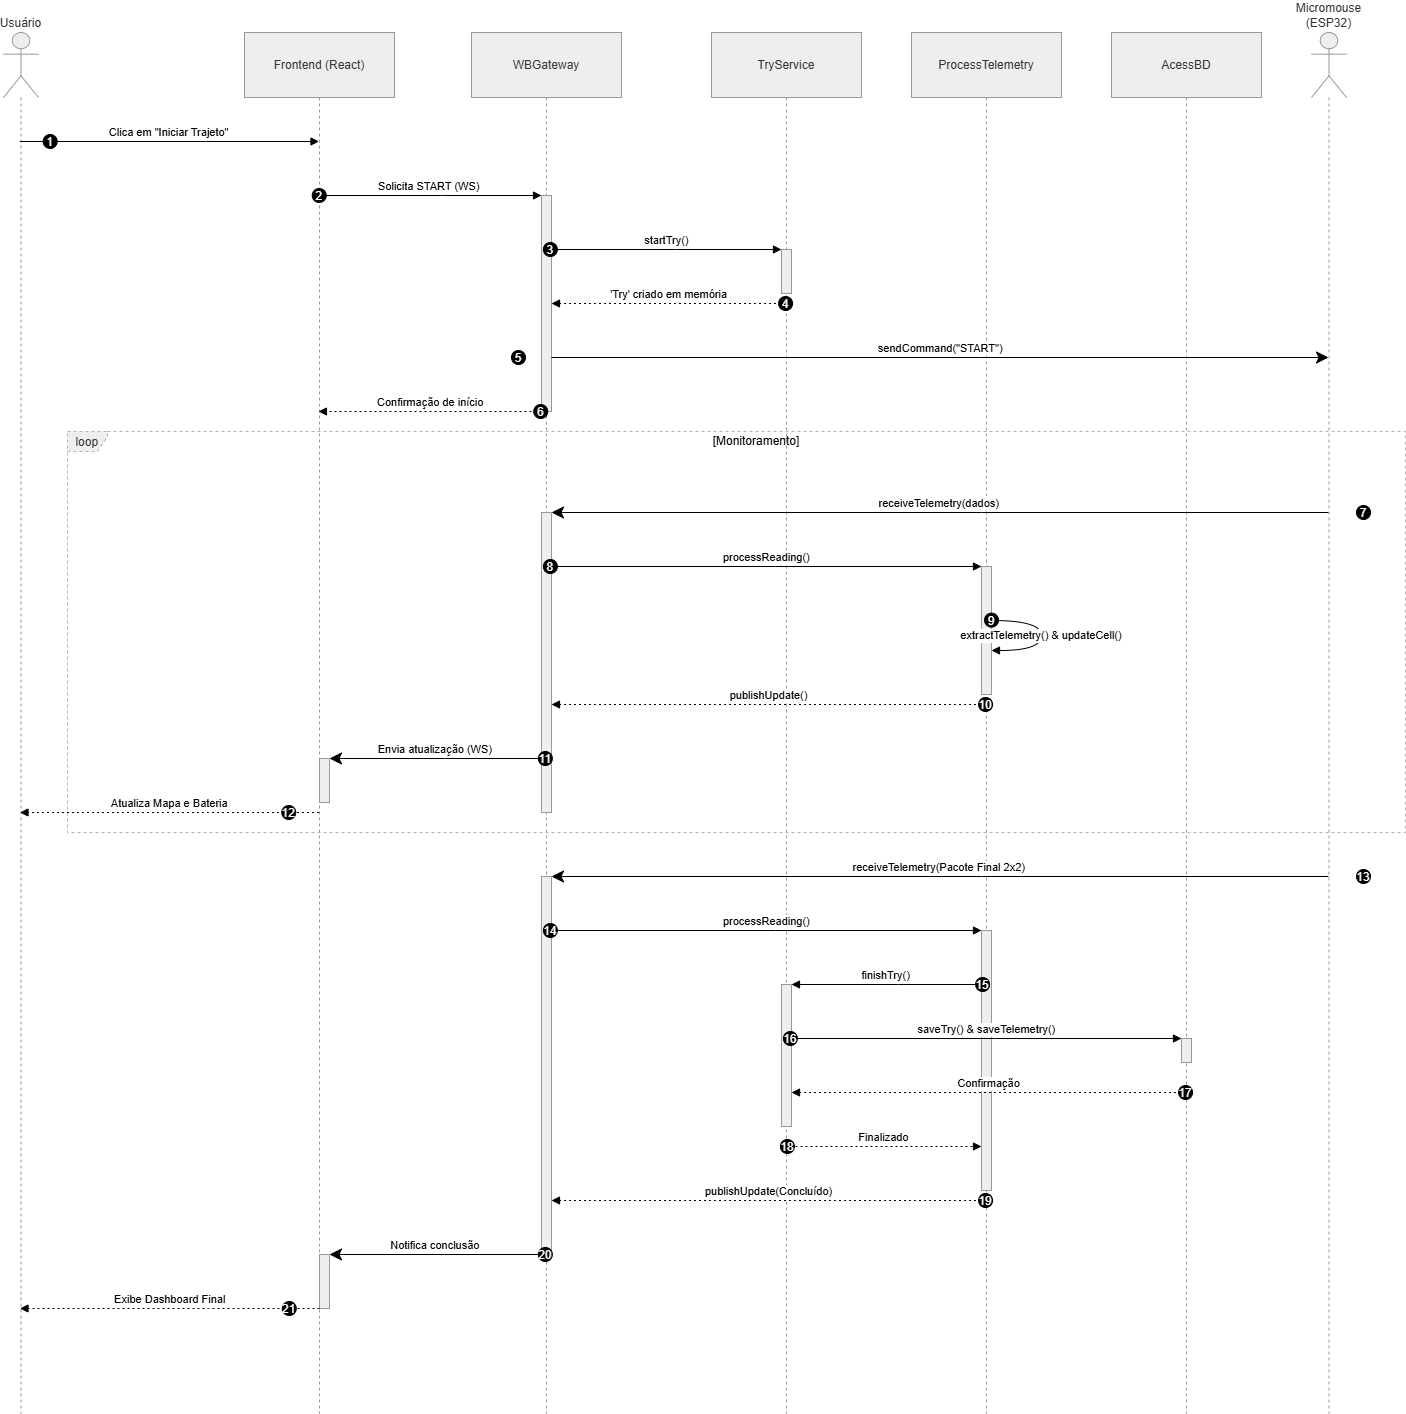
\includegraphics[width=\textwidth]{figuras/software/seq_execucao.png}
    \caption{Diagrama de Sequência: Fluxo de Execução Principal.}
    \label{fig:seq_execucao}
\end{figure}

O \textbf{Cenário de Interrupções} (Figura \ref{fig:seq_interrupcao}) mapeia a resiliência do software diante de eventos assíncronos. O diagrama ilustra o tratamento de comandos de parada manual e reinicialização enviados pelo usuário, garantindo que o estado da aplicação permaneça consistente mesmo em abortos inesperados de trajeto.

\begin{figure}[H]
    \centering
    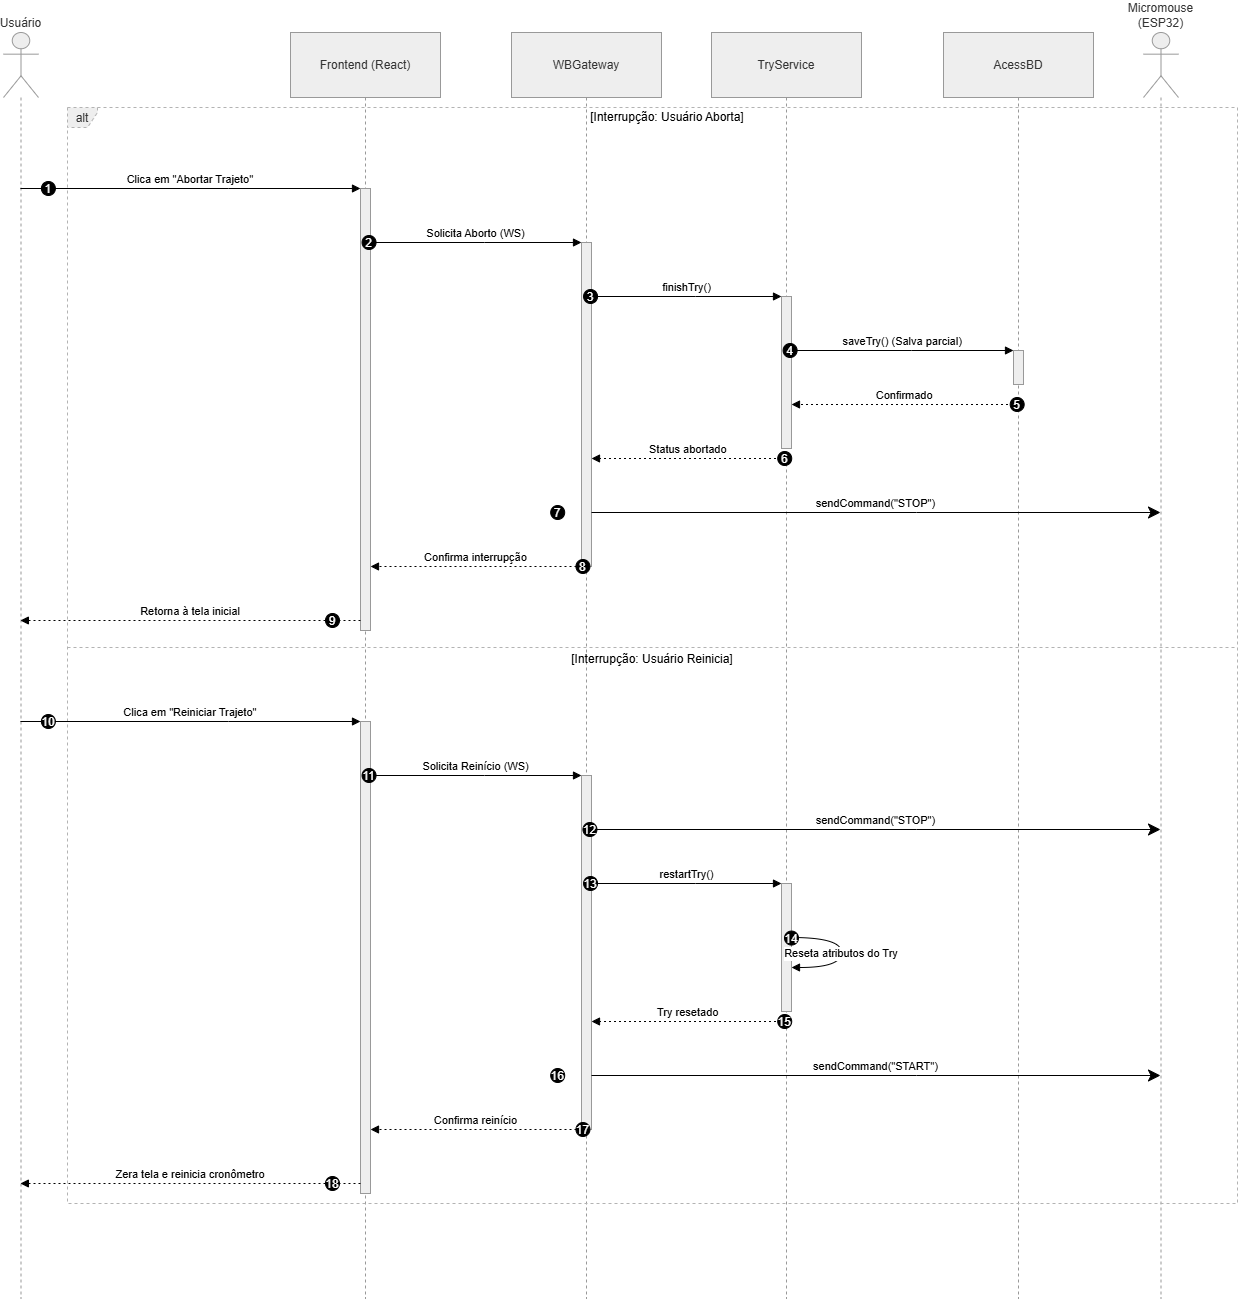
\includegraphics[width=\textwidth]{figuras/software/seq_interrupcao.png}
    \caption{Diagrama de Sequência: Fluxo de Interrupções e Resets.}
    \label{fig:seq_interrupcao}
\end{figure}

Por fim, o \textbf{Cenário de Consulta ao Histórico} (Figura \ref{fig:seq_historico}) detalha a recuperação de dados persistidos. O fluxo demonstra a comunicação entre o \textit{frontend} e o banco de dados para a renderização de trajetos passados, permitindo a análise de desempenho do robô após as corridas.

\begin{figure}[H]
    \centering
    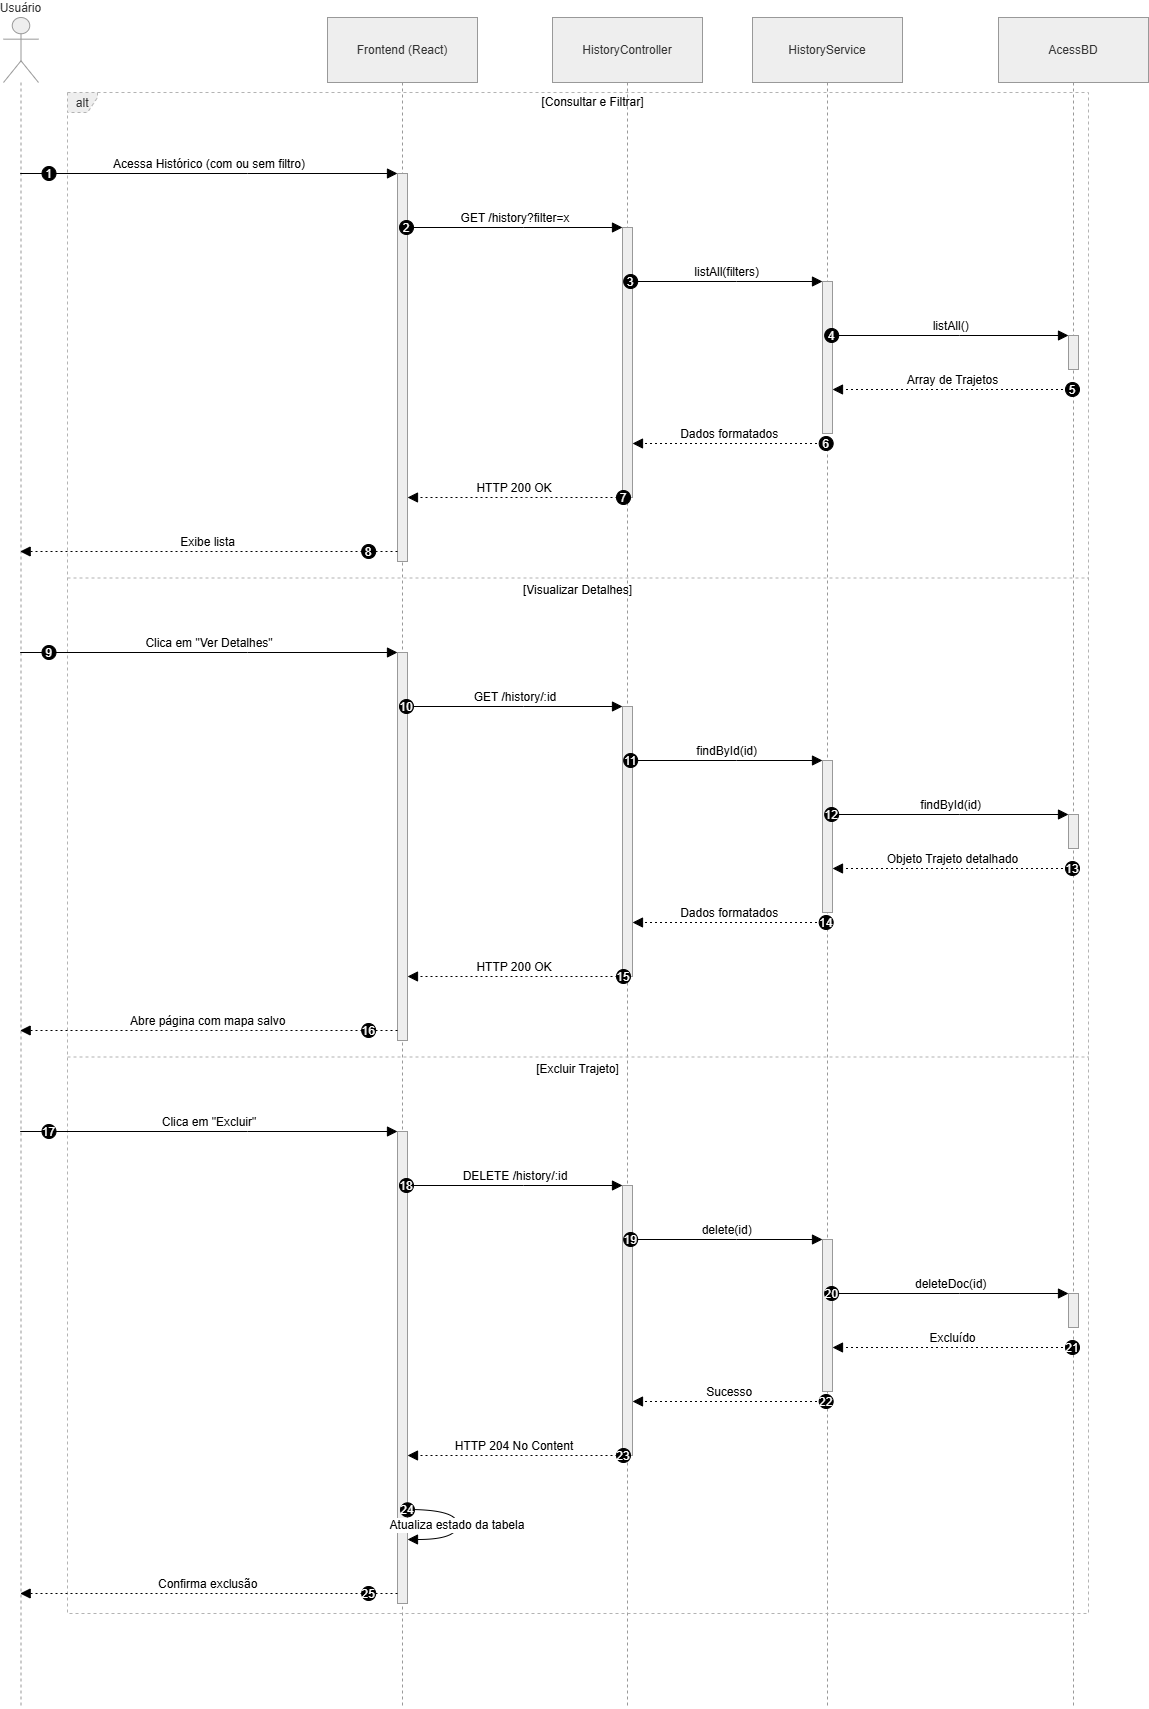
\includegraphics[width=\textwidth]{figuras/software/seq_historico.png}
    \caption{Diagrama de Sequência: Recuperação de Histórico.}
    \label{fig:seq_historico}
\end{figure}

\subsection{Visão de Implementação do Software}

\subsubsection{Diagrama de Componentes}

\subsubsection{Diagrama de Pacotes}
    O diagrama de pacotes (Figura \ref{fig:diagrama_pacotes_sw}) descreve os relacionamentos de dependência entre um pacote para outro, mostrado a disposição de cada elemento de modelo e esclarecer a estrutura hierárquia dos elementos.

    A estrutura é dividida em Frontend, representa a aplicação da interface, dividida em módulos como de componentes, lógica e comunicação, Backend, representa a comunicação entre esses dados, dividida em módulos como de telemetria e controle, EPS32, detalha o software que roda no \textit{micromouse}, dividido em módulos como de Navegação e serviço WiFi, e Firebase, que é uma camada externa utilizada para guardar os dados.
    \begin{figure}[H]
        \centering
        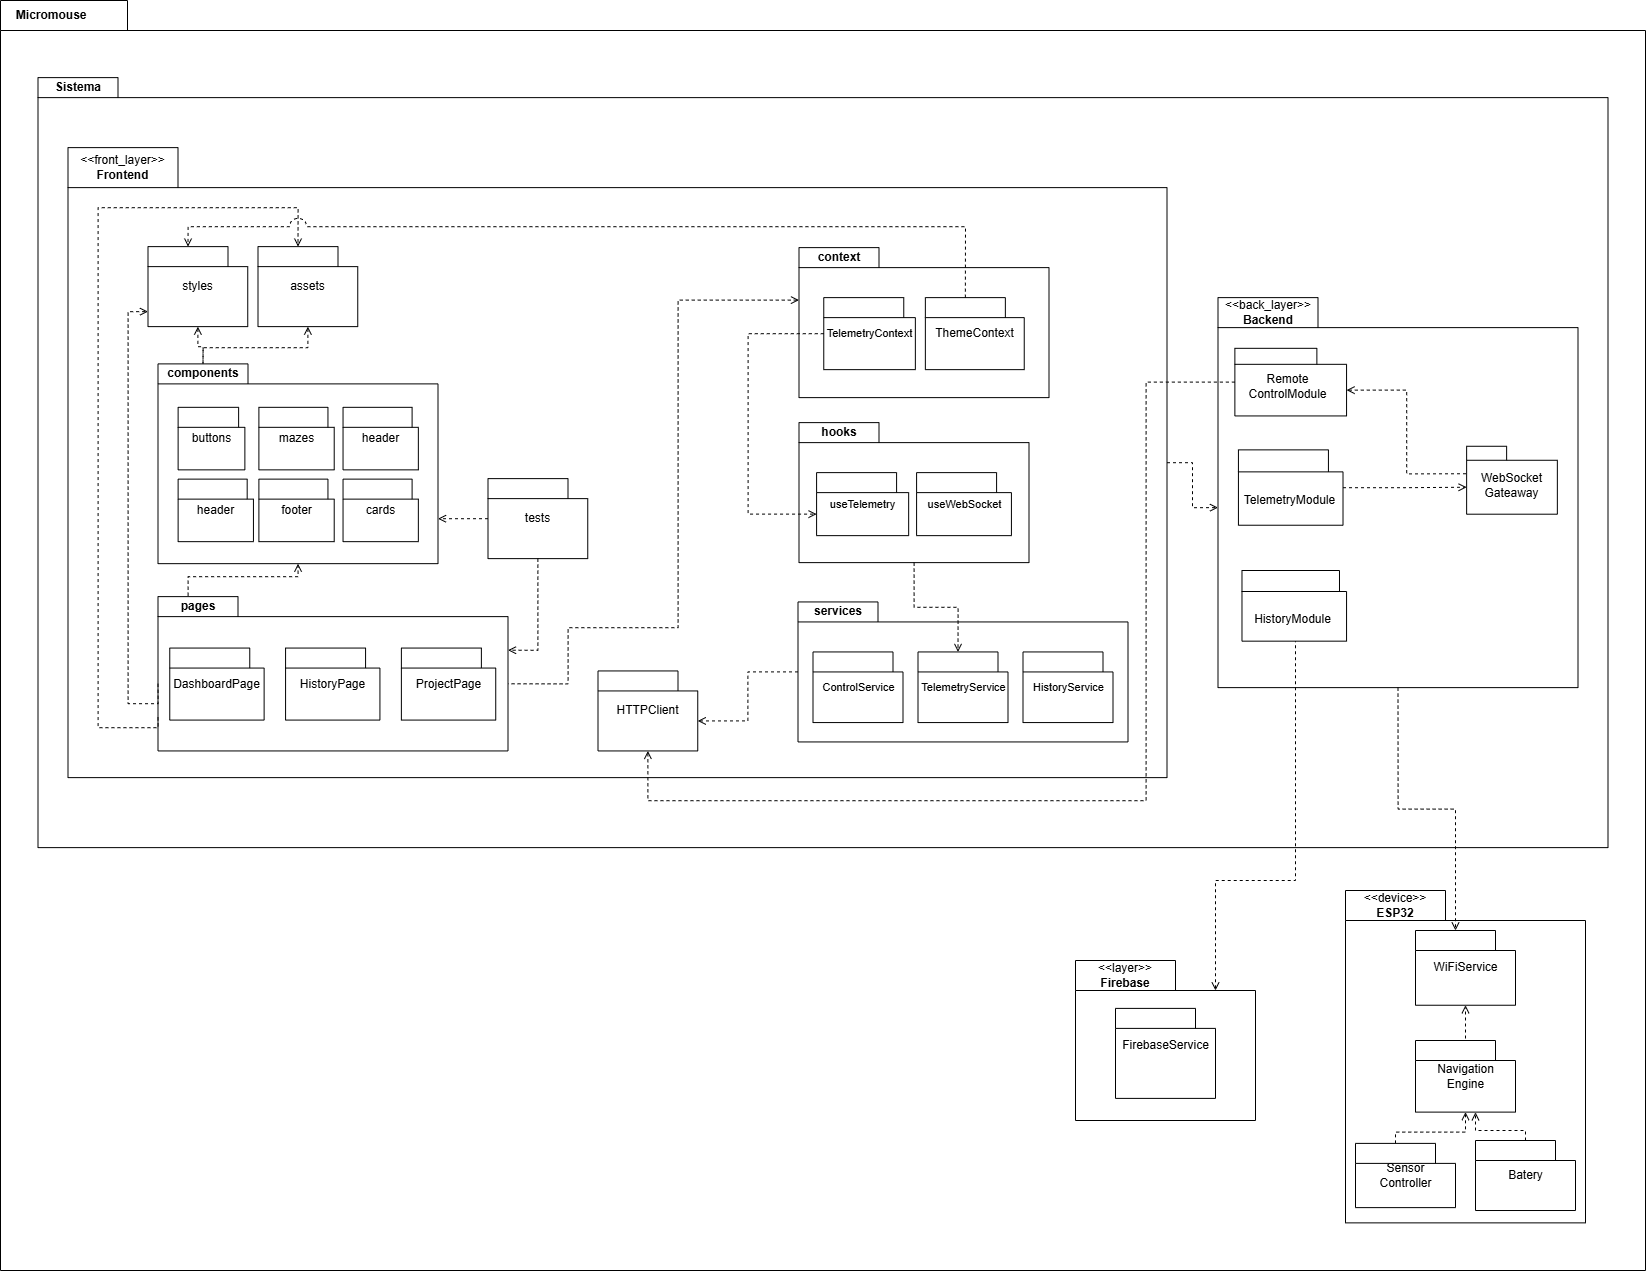
\includegraphics[width=\textwidth]{figuras/software/diagrama-de-pacotes.png}
        \caption{Diagrama de Pacotes.}
        \label{fig:diagrama_pacotes_sw}
    \end{figure}

\subsection{Visão de Implantação do Software}
\subsubsection{Diagrama de Implantação}

\begin{figure}[H]
    \centering
    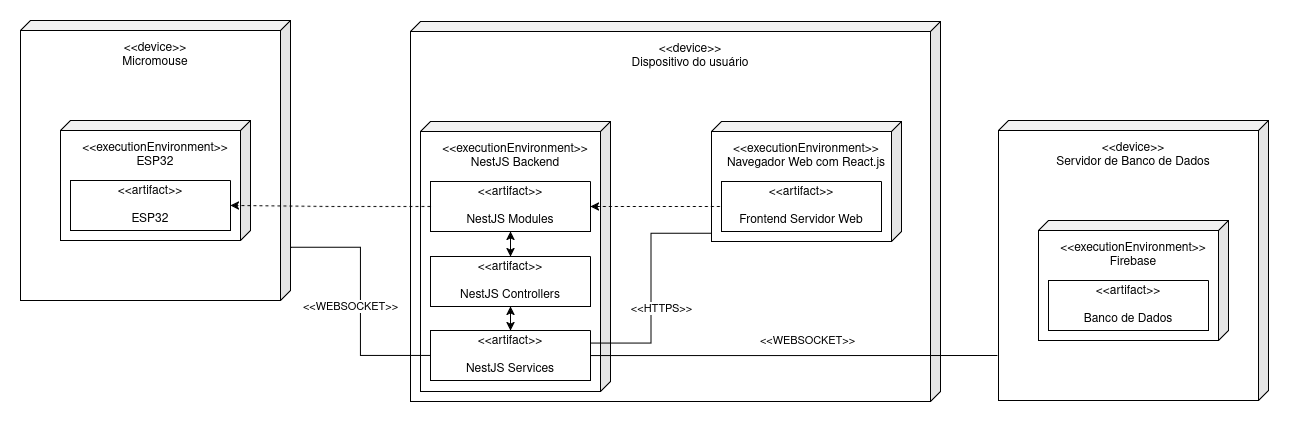
\includegraphics[width=0.8\textwidth]{figuras/software/diagrama_implantacao.png}
    \captionsetup{font=footnotesize}
    \caption{Diagrama de implantação do sistema.}
    \label{fig:diagrama_implantacao}
\end{figure}

A Fig.~\ref{fig:diagrama_implantacao} demonstra a arquitetura do sistema, caminhos de comunicação entre o \textit{Micromouse}, o sistema web, e o banco de dados, e como esses subsistemas se dispõem entre o rato físico, o dispositivo do usuário, e o serviço de banco de dados.

A comunicação entre os subsistemas acontece principalmente através de \textit{WebSocket} a fim de possibilitar o acompanhamento em tempo real da navegação do \textit{micromouse}; essa mesma razão justifica a escolha do \textbf{Firebase Realtime Database} como serviço de banco de dados. No \textit{micromouse} e back-end do servidor web, essa conexão é facilitada por módulo incluso na \textbf{ESP32} e a framework \textbf{NestJS}, respectivamente.

Como espera-se que o back-end e o front-end do servidor web sejam executados na mesma máquina (dispositivo do usuário), a conexão por \textit{HTTPS} foi determinada como suficiente para o funcionamento da interface de usuário.

O diagrama mostra também a relação de dependência entre o back-end e o \textit{micromouse} — indicando que o rato é capaz de operar independentemente — e entre o front-end e o back-end. 

\subsection{Visão de Dados do Software} 

A Visão de Dados descreve a forma como as informações geradas, processadas e consumidas pelo sistema são estruturadas e armazenadas. Tendo em vista as características do projeto, que exige alta taxa de transferência e armazenamento de dados de telemetria em tempo real, optou-se pela utilização do Firebase, um banco de dados NoSQL orientado a documentos que armazena os dados em coleções, as quais contêm documentos que podem abrigar subcoleções.

\subsubsection{Diagrama de Estrutura de Documentos} 
    Na Figura \ref{fig:diagrama_estrutura_documentos}, temos o Diagrama de Estrutura de Documentos que reflete a modelagem escolhida para otimizar as consultas do sistema web. A base de dados está dividida em duas coleções principais:

    \begin{itemize}
        \item \textbf{Coleção Labirinto:} Responsável por armazenar a estrutura física e lógica do labirinto percorrido. Cada documento representa um labirinto específico e possui atributos como \textit{id} e \textit{status}, além de uma subcoleção \textit{Nos} e uma subcoleção de metadados para dimensionamento.
        \item \textbf{Coleção Tentativa:} Responsável por armazenar o registro de telemetria do Micromouse. Cada vez que o robô inicia um percurso, um novo documento é criado nesta coleção, contendo atributos da tentativa e subcoleções específicas para os dados de velocidade e de bateria.
    \end{itemize}


    \begin{figure}[H]
        \centering
        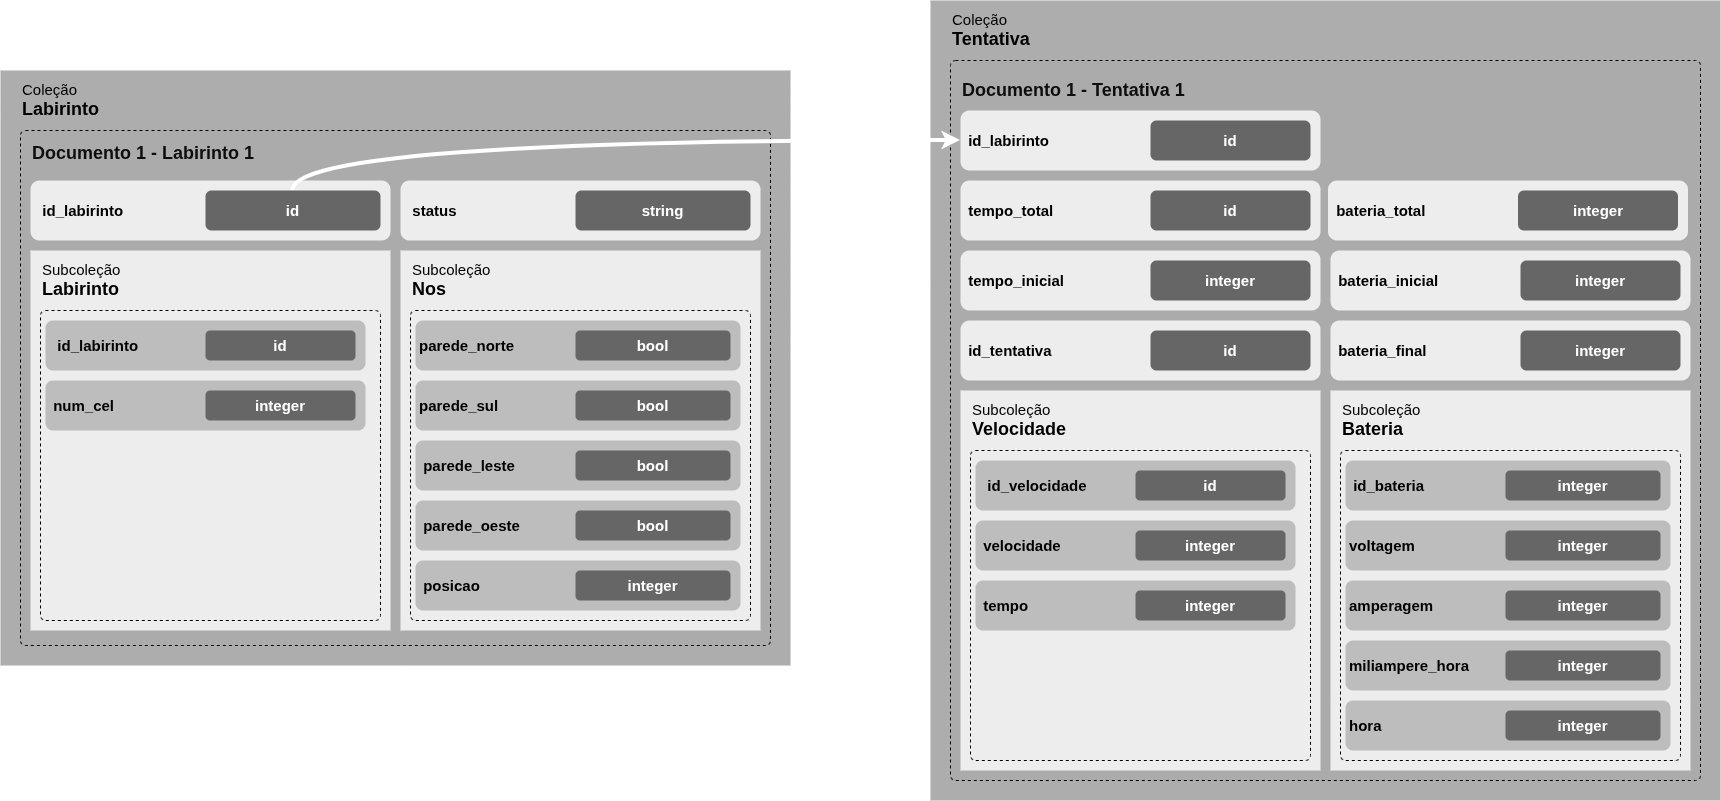
\includegraphics[width=\textwidth]{figuras/software/diagrama_estrutura_documentos.png}
        \caption{Diagrama de Estrutura de Documentos.}
        \label{fig:diagrama_estrutura_documentos}
    \end{figure}

    \subsection{Roteiro de testes funcionais}

    Os roteiro de testes funcionais pode ser observado na Tabela \ref{tab:roteiro_testes_funcionais}

    \begin{table}[H]
        \centering
        \caption{Casos de testes funcionais}
        \label{tab:roteiro_testes_funcionais}
        \footnotesize
        \begin{tabular}{|p{0.9cm}|p{2.3cm}|p{2.3cm}|p{3cm}|p{3cm}|p{3.2cm}|}
        \hline
        Id   & Nome                                & Objetivo                                                               & Pré-condições                                                                                                                                                            & Procedimentos                                                                                                                                                              & Pós-condições                                                                                                                                                                      \\ \hline
        CT01 & Monitoramento do percurso           & Validar a exibição e recebimento dos dados de telemetria do micromouse & Micromouse navegando no labirinto, servidor aberto e rodando a aplicação Web e micromouse conectado ao servidor via websocket & Iniciar o percurso e e Observar a interface web durante a execução                                                               & A interface web deve atualizar em tempo real as informações: posição no labirinto, amperagem da bateria, voltagem da bateria, velocidade, tempo da execução e status da tentativa. \\ \hline
        CT02 & Comandos remotos                    & Validar comandos remotos para o micromouse                             & Servidor aberto e rodando a aplicação Web e micromouse conectado ao servidor via websocket                                      & Apertar botão de “iniciar”, confirmar início da execução, apertar botão de “reiniciar”, confirmar reinício da execução & O sistema deve iniciar a tentativa no labirinto e o cronômetro, resetá-lo ao reiniciar.                                                                                           \\ \hline
        CT03 & Finalização e métricas da tentativa & Validar processamento dos dados ao término da tentativa                & Servidor aberto e rodando a aplicação Web, micromouse conectado ao servidor via websockete e tentativa em andamento.            & Executar a tentativa até a finalização, interrupção ou falhae e observar tela final                                              & A interface web deve informar falha/sucesso e exibir as informações médias da tentativa                                                                                           \\ \hline
        CT04 & Armazenamento de dados              & Validar o salvamento de informações após o término da tentativa.       & Servidor aberto e rodando a aplicação Web, micromouse conectado ao servidor via websockete e tentativa finalizada               & Finalizar a tentativae e consultar a tentativa no banco                                                                          & Os dados devem ser armazenados no banco de dados sem nenhuma perda de informação                                                                                                   \\ \hline
        CT05 & Consulta de histórico               & Validar consulta de tentativas anteriores.                             & Servidor aberto e rodando a aplicação Web e existência de registros salvos no banco.                                            & Pesquisar uma tentativa e clicar para visualização                                                                             & Os dados devem ser apresentados em tela sem nenhuma perda de informação para qualquer tipo de labirinto \\ \hline
        \end{tabular}
    \end{table}

    
    % \textcolor{red}{Itens fundamentais:}
    % \begin{itemize}
    %     \item \textcolor{red}{\textbf{\textit{Backlog} do Produto}}
    %     \begin{itemize}
    %         \item \textcolor{red}{ Descrever os requisitos funcionais (RF) com a técnica de documentação e especificação de história de usuário (HU);}
    %         \item \textcolor{red}{ Descrever os requisitos não-funcionais (RNF) de forma objetiva; Mais facilmente, mais rapidamente, mais responsivo, de fácil uso, são descrições subjetivas não-válidas. Um exemplo de requisito não-funcional de desempenho: ``a página deve carregar em até 5s quando em conexão 4G''.}
    %         \item \textcolor{red}{ Ao descrever os requisitos (RF e RNF), usar a classificação MoSCoW (\textit{Must have}, \textit{Should have} e \textit{Could have}), para auxiliar a priorização dos itens do backlog.}
    %         \item \textcolor{red}{ Protótipos de interface gráfica do \textit{software} em alta fidelidade.}
    %     \end{itemize}
    % \end{itemize}

    % \begin{itemize}
    % \item \textcolor{red}{ \textbf{Descrição da arquitetura da solução de \textit{software} proposta:}}
    
    %     \item \textcolor{red}{ Esta subseção deve contemplar o documento de arquitetura do sistema e deve ser estruturado segundo as visões (4+1) previstas no processo unificado (UP): lógica, de processos;  implementação, implantação e dados (substuirá a visão de casos de uso).}
        
    %     \item \textcolor{red}{ Propósito do \textit{software} (qual o seu papel no sistema);}
    %     \item \textcolor{red}{ Padrão adotado : MVC, MVP, Microsserviços, Monolítico, etc (Justificar);}
    %     \item \textcolor{red}{ Linguagens de programação: Java, Python, C\#, JavaScript, etc.}
    %     \item \textcolor{red}{ \textit{Frameworks} e bibliotecas: Spring Boot, .NET Core, React, Angular, Django, etc.}
    %     \item \textcolor{red}{ Banco de dados: Relacional (PostgreSQL, MySQL, etc) X NãoSQL (MongoDB,etc). }
    %     \item \textcolor{red}{Persistência de dados: Modelo Entidade‑Relacionamento (MER) e seu respectivo Diagrama Entidade‑Relacionamento (DER), aplicáveis quando a solução utiliza banco de dados relacional; alternativamente, diagrama de estrutura de documentos, empregado nos casos em que a arquitetura adota banco de dados não relacional.}
    % \end{itemize}  

    % \begin{itemize}
    % \item \textcolor{red}{\textbf{ Roteiro de testes funcionais:} }
    %     \item \textcolor{red}{Código do caso de teste;}
    %     \item \textcolor{red}{Nome do caso de teste;}
    %     \item \textcolor{red}{ Objetivo do caso de teste;}
    %     \item \textcolor{red}{ Pré-condições do sistema para o teste ser realizado, quando se aplicar;}
    %     \item \textcolor{red}{ Descrição dos procedimentos a serem executados para o teste;}
    %     \item \textcolor{red}{ Resultado esperado para o teste ser aprovado (pós-condição após realizado o teste);}
    % \end{itemize}
% \end{itemize}

